\documentclass[12pt,letterpaper]{article}
\usepackage[utf8]{inputenc}
\usepackage[spanish]{babel}
\usepackage{graphicx}
\usepackage[left=2cm,right=2cm,top=2cm,bottom=2cm]{geometry}
\usepackage{graphicx} % figuras
% \usepackage{subfigure} % subfiguras
\usepackage{float} % para usar [H]
\usepackage{amsmath}
%\usepackage{txfonts}
\usepackage{stackrel} 
\usepackage{multirow}
\usepackage{enumerate} % enumerados
\renewcommand{\labelitemi}{$-$}
\renewcommand{\labelitemii}{$\cdot$}
% \author{}
% \title{Caratula}
\begin{document}

% Fancy Header and Footer
% \usepackage{fancyhdr}
% \pagestyle{fancy}
% \cfoot{}
% \rfoot{\thepage}
%

% \usepackage[hidelinks]{hyperref} % CREA HYPERVINCULOS EN INDICE

% \author{}
\title{Caratula}

\begin{titlepage}
\begin{center}
\large{UNIVERSIDAD PRIVADA DE TACNA}\\
\vspace*{-0.025in}
\begin{figure}[htb]
\begin{center}

\includegraphics[width=8cm]{./Imagenes/logo}
\end{center}
\end{figure}
\vspace*{0.15in}
INGENIERIA DE SISTEMAS  \\

\vspace*{0.5in}
\begin{large}
TITULO:\\
\end{large}

\vspace*{0.1in}
\begin{Large}
\textbf{PRACTICA DE LABORATORIO N 02} \\
\textbf{Modelando Datos en Power BI} \\
\end{Large}

\vspace*{0.3in}
\begin{Large}
\textbf{CURSO:} \\
\end{Large}

\vspace*{0.1in}
\begin{large}
INTELIGENCIA DE NEGOCIOS\\
\end{large}

\vspace*{0.3in}
\begin{Large}
\textbf{DOCENTE(ING):} \\
\end{Large}

\vspace*{0.1in}
\begin{large}
 Patrick Cuadros Quiroga\\
\end{large}

\vspace*{0.2in}
\vspace*{0.1in}
\begin{large}
Integrante: \\
\begin{flushleft}
Mamani Limache, Jhony 		\hfill	(2013046566) 
\end{flushleft}
\end{large}
\end{center}

\end{titlepage}


\tableofcontents % INDICE
\thispagestyle{empty} % INDICE SIN NUMERO
\newpage
\setcounter{page}{1} % REINICIAR CONTADOR DE PAGINAS DESPUES DEL INDICE


\begin{center}
    PRACTICA DE LABORATORIO N° 02
\end{center}

\section{OBJETIVOS}
A.

\section{REQUERIMIENTOS}

\begin{itemize}

- Conocimientos básicos de administración de base de datos Microsoft   SQL Server.
\\- Conocimientos básicos de SQL.
\\- Microsoft SQL Server 2016 o superior
\\- Base de datos AdventureWorks2016 o superior
\\- Power BI Desktop.
\\- Tener una cuenta Microsoft registrada en el Portal de Power Bi.
\end{itemize}

\section{DESARROLLO} 

\begin{itemize}
    Ejercicio 1: Crear relaciones \\\\
    Tarea 1: Relaciones automáticas\\\\
    1.  Ingresar a Power BI Desktop.\\
    2.  En la Ventana de Power BI Desktop, click en Obtener Datos (Get Data)\\
    3.  En el cuadro de dialogo Obtener Datos (Get Data), asegurarse que Excel esta seleccionado y hacer click
        en Conectar (Connect).\\
    4.  En el cuadro de dialogo Abrir (Open), buscar el archivo Adventure Works Sales Data.xlsx, y luego hacer
click en Abrir (Open).\\
    5.  En el cuadro de dialogo Explorador (Navigator), seleccionar las hojas DimCurrency, DimCustomer,
DimDate, DimProduct, DimPromotion, DimSalesTerritory, y FactInternetSales.\\
    6.  Hacer click en Cargar (Load)\\

\end{itemize} 

\begin{center}
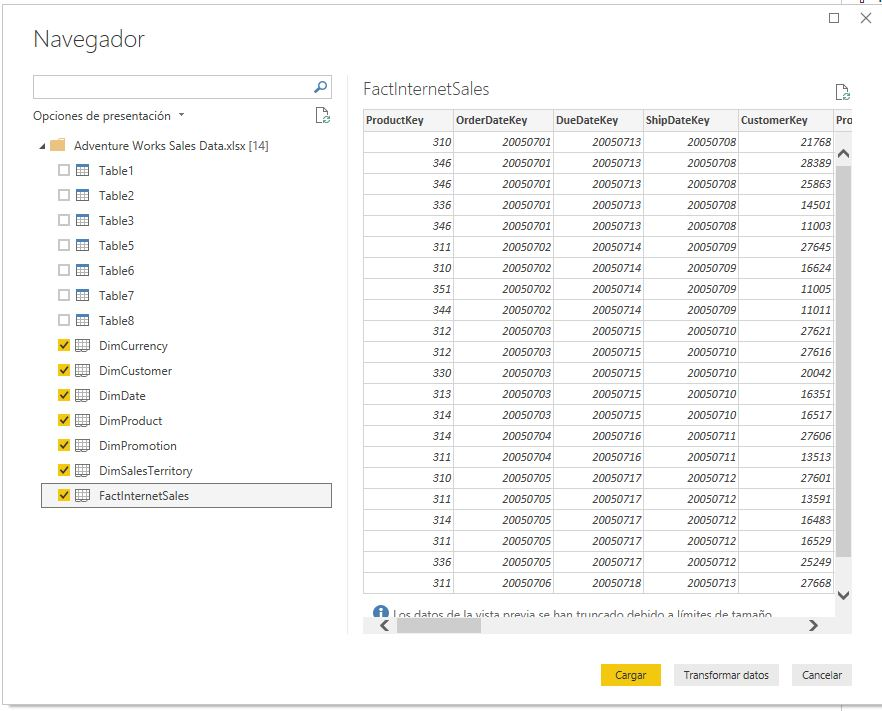
\includegraphics[width=12cm]{./Imagenes/img1-6} 
\end{center}
    
\begin{itemize}
    7.  En el panel de vistas a mano derecho, hacer click en Relaciones (Relationships)\\
    8.  En el menú principal, hacer click en Administrar relaciones (Manage Relationships).\\

\end{itemize} 


\begin{center}
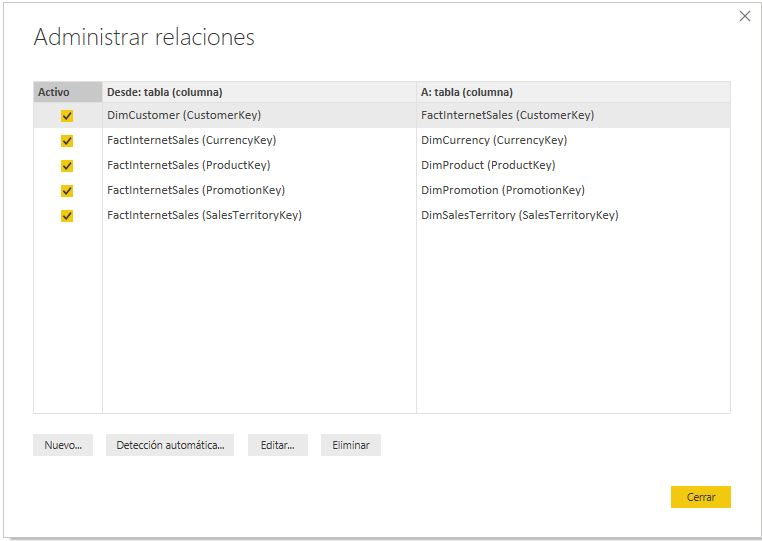
\includegraphics[width=12cm]{./Imagenes/img7-8} 
\end{center}
    
      
\begin{itemize}
    9.  En el cuadro de Administrar relaciones (Manage Relationships), hacer click en Nueva (New)\\
    10.  En el cuadro de Administrar relaciones (Manage Relationships), en la lista de tablas superior, hacer         click en FactInternetSales. Cuando la vista previa de la table aparezca hacer click en la columna            OrderDateKey\\
    11. En la lista de table inferior, hacer click en DimDate. Cuando la vista previa de la table aparezca hacer     click en la columna DateKey.\\
    12. Revisar que la cardinalidad (Cardinality) esta seleccionada para Muchos a Uno (Many to One (*:1)), que la
Dirección del filtro cruzado (Cross filter direction) es Sencilla (Single), y que la opción Hacer esta relación
activa (Make this relationship active) se encuentra seleccionada, luego hacer click en Aceptar (OK).\\

\end{itemize} 

\begin{center}
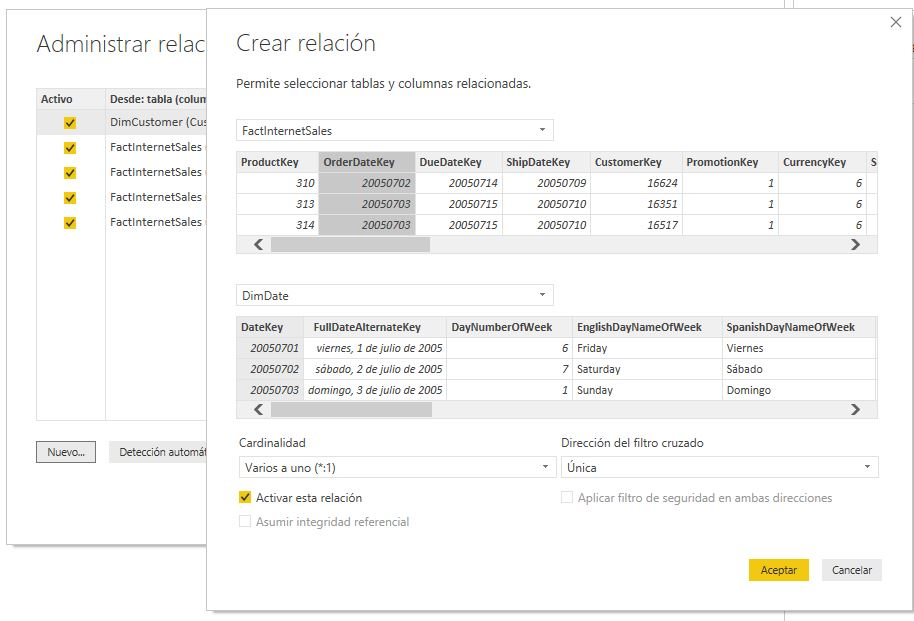
\includegraphics[width=12cm]{./Imagenes/img9-12} 
\end{center}
    
    
        
\begin{itemize}
    13.  \\
    14. \\
    15. \\
    16. \\
    17.  \\
    18. \\
    19. \\
    20. \\
    21.  \\
    22. \\
    23. \\
    24. \\
    25.  \\
    26. \\
    27. \\
    28. \\
    29.  \\
    30. \\
    31. \\
    32. \\
    33.  \\
    34. \\

\end{itemize} 
    
\begin{center}
\includegraphics[width=12cm]{./Imagenes/img13-34} 
\end{center}
    
      
\begin{itemize}
   Tarea 2: Relaciones manuales\\\\
   1.   En la Ventana de Power BI Desktop, click en Obtener Datos (Get Data) y luego en Excel\\
   2.   Abrir el archivo Adventure Works Product Categories.xlsx.\\
   3.   En el cuadro de dialogo Explorador (Navigator), seleccionar las hojas DimProductCategory, and
DimProductSubcategory, y luego hacer click en Cargar (Load).\\
   
\end{itemize} 

    
\begin{center}
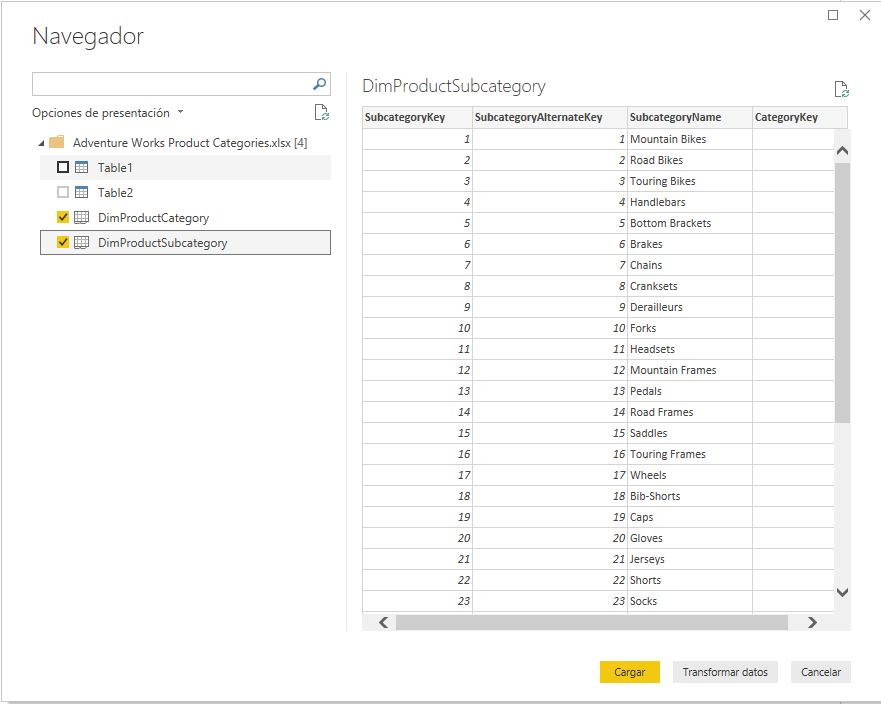
\includegraphics[width=12cm]{./Imagenes/img2-1-3} 
\end{center}
   
     
\begin{itemize}
   4.   En el panel de Relaciones, revisar la relación que Power BI ha creado entre las dos tablas.\\
   5.   Hacer click en la línea de la relación entre DimProductCategory, y DimProductSubcategory, y seleccionar Eliminar (Delete)\\
   
\end{itemize} 

    
\begin{center}
\includegraphics[width=12cm]{./Imagenes/img2-4-5} 
\end{center}
    
    
    
    
    
\include{Secciones/Actividad02}
\include{Secciones/Actividad03}
\include{Secciones/Actividad04}




\end{document}
